\newcommand{\commonCrawlFilesTable}[0]{
    \renewcommand\arraystretch{1.2}
    % Please add the following required packages to your document preamble:
    % \usepackage{graphicx}
    % \usepackage[table,xcdraw]{xcolor}
    % If you use beamer only pass "xcolor=table" option, i.e. \documentclass[xcolor=table]{beamer}
    \begin{table}[h]
    \resizebox{\textwidth}{!}{%
    \begin{tabular}{lllr}
    \rowcolor[HTML]{C0C0C0} 
    Tipo File                                                          & Descrizione                                                                                                                                              & \#Files & \begin{tabular}[c]{@{}r@{}}Dim.dei file\\ compressi\end{tabular} \\ \hline
    \rowcolor[HTML]{EFEFEF} 
    Segments                                                           &                                                                                                                                                          & 100     &                                                                   \\
    WARC files                                                         & Dati grezzi generati dal Crawler                                                                                                                         & 64000   & 59.86 TiB                                                         \\
    \rowcolor[HTML]{EFEFEF} 
    WAT files                                                          & \begin{tabular}[c]{@{}l@{}}Contengono meta-dati relativi ai record nei \\ file WARC\end{tabular}                                                          & 64000   & 18.23 TiB                                                         \\
    WET files                                                          & \begin{tabular}[c]{@{}l@{}}Contengono solo testo semplice estratto \\ dai WARC\end{tabular}                                                              & 64000   & 7.62 TiB                                                          \\
    \rowcolor[HTML]{EFEFEF} 
    Robots.txt files                                                   & \begin{tabular}[c]{@{}l@{}}Files Robot.txt richiesti ai vari siti analizzati \\ (consentono al Crawler di scansionare \\ meglio i siti web)\end{tabular} & 64000   & 170 GiB                                                          \\
    \begin{tabular}[c]{@{}l@{}}Non-200 \\ responses files\end{tabular} & \begin{tabular}[c]{@{}l@{}}Risposte del server con HTTP status code \\ diverso da 200 (404, redirects, ecc.)\end{tabular}                                & 64000   & 1.79 TiB                                                          \\
    \rowcolor[HTML]{EFEFEF} 
    URL index files                                                    & \begin{tabular}[c]{@{}l@{}}Indice degli url analizzati, completo di utili \\ informazioni aggiuntive\end{tabular}                                        & 302     & 210 GiB                                                         
    \end{tabular}%
    }
    \end{table}
    \renewcommand\arraystretch{1.0}
}

%TOTALE: 88791
%tick: 49668
%x: 5371
%plus: 14058
%minus: 14941
%divided: 4753
\newcommand{\printHistogram}[0]{
    %\pgfplotsset{scaled y ticks=false}
    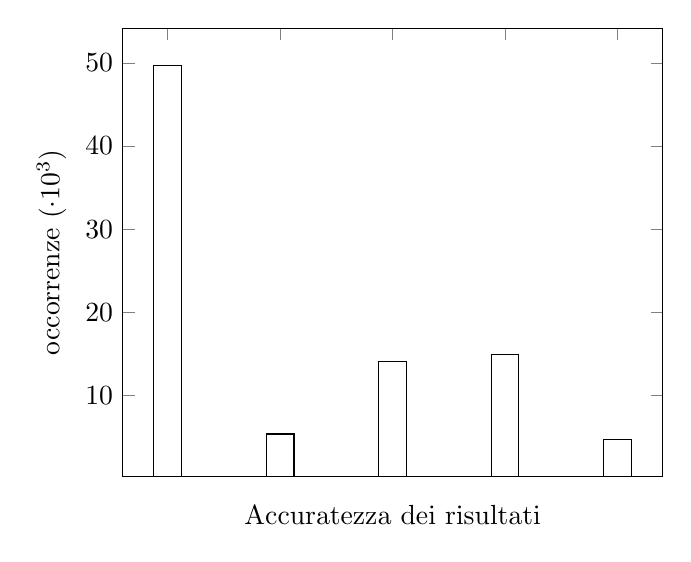
\begin{tikzpicture}
    \begin{axis}[
        symbolic x coords={\imgtick{},\imgx{},\imgplus{},\imgminus{},\imgdivided{}}, 
        ylabel = {occorrenze ($\cdot 10^3$)}, 
        xlabel = {Accuratezza dei risultati}, 
        xtick=data]
        
        \addplot[ybar,fill=white] coordinates {
            (\imgtick{}, 49.668)
            (\imgx{}, 5.371)
            (\imgplus{}, 14.058)
            (\imgminus{}, 14.941)
            (\imgdivided{}, 4.753)
        };
    \end{axis}
    \end{tikzpicture}
}

\newcommand{\printTimeGraph}[0]{
    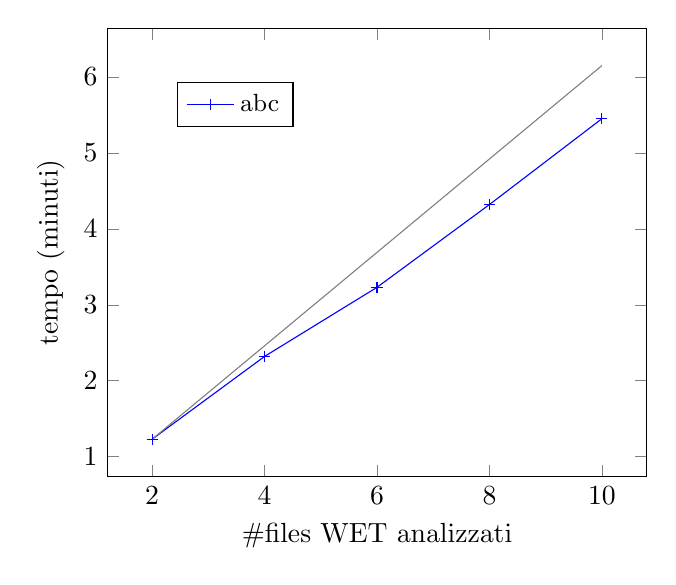
\begin{tikzpicture}
    \begin{axis}[
      %ymin=20,
      %ymax=90,
      %width=15cm,
      %height=7cm,
      ylabel={tempo (minuti)},
      xlabel={\#files WET analizzati},
      %xticklabels={,2,4,6,8,10}, 
      legend style={at={(0.13,0.83)},
      anchor=west, legend columns=-1, font=\small},
      legend cell align=left,
      xtick=data
     ]

    \addlegendentry{abc}

    \addplot[blue, mark=+] coordinates {
        (2, 1.23)
        (4, 2.32)
        (6, 3.23)
        (8, 4.32)
        (10, 5.45)
    };
    
    \addplot[gray, mark=] coordinates {
        (2, 1.23)
        (4, 2.46)
        (6, 3.69)
        (8, 4.92)
        (10, 6.15)
    };
    \end{axis}
    \end{tikzpicture}
}